
\documentclass[a4paper,11pt]{article}%,twocolumn
%% packages

\usepackage{blindtext} % needed for creating dummy text passages
%\usepackage{ngerman} % needed for German default language
\usepackage{amsmath} % needed for command eqref
\usepackage{amssymb} % needed for math fonts
\usepackage[colorlinks=true,breaklinks]{hyperref} % needed for creating hyperlinks in the document, the option colorlinks=true gets rid of the awful boxes, breaklinks breaks lonkg links (list of figures), and ngerman sets everything for german as default hyperlinks language
\usepackage[hyphenbreaks]{breakurl} % ben�tigt f�r das Brechen von URLs in Literaturreferenzen, hyphenbreaks auch bei links, die �ber eine Seite gehen (mit hyphenation).
\usepackage{xcolor}
\definecolor{c1}{rgb}{0,0,1} % blue
\definecolor{c2}{rgb}{0,0.3,0.9} % light blue
\definecolor{c3}{rgb}{0.3,0,0.9} % red blue
\hypersetup{
    linkcolor={c1}, % internal links
    citecolor={c2}, % citations
    urlcolor={c3} % external links/urls
}
%\usepackage{cite} % needed for cite
\usepackage[square,authoryear]{natbib} % needed for cite and abbrvnat bibliography style
\usepackage[nottoc]{tocbibind} % needed for displaying bibliography and other in the table of contents
\usepackage{graphicx} % needed for \includegraphics 
\usepackage{longtable} % needed for long tables over pages
\usepackage{bigstrut} % needed for the command \bigstrut
\usepackage{enumerate} % needed for some options in enumerate
%\usepackage{todonotes} % needed for todos
\usepackage{makeidx} % needed for creating an index
\makeindex
\usepackage{gensymb}
\usepackage{url}
\usepackage{psfrag}
\usepackage{multirow}
\usepackage{subfigure}
%% page settings

\usepackage[top=20mm, bottom=20mm,left=15mm,right=15mm]{geometry} % needed for page border settings
\parindent=0mm % for space of first line of new text block
\sloppy % for writing with hyphenless justification (tries to)
\hyphenation{} % use hyphenation of tolerance parametershttp://www.jr-x.de/publikationen/latex/tipps/zeilenumbruch.html
\hyphenpenalty=10000
\exhyphenpenalty=10000
\usepackage{fancyhdr} % needed for head and foot options
%% my macros

%% Text fomats
\newcommand{\tbi}[1]{\textbf{\textit{#1}}}

%% Math fonts
\newcommand{\bbA}{\mathbb{A}}
\newcommand{\bbB}{\mathbb{B}}
\newcommand{\bbC}{\mathbb{C}}
\newcommand{\bbD}{\mathbb{D}}
\newcommand{\bbE}{\mathbb{E}}
\newcommand{\bbF}{\mathbb{F}}
\newcommand{\bbG}{\mathbb{G}}
\newcommand{\bbH}{\mathbb{H}}
\newcommand{\bbI}{\mathbb{I}}
\newcommand{\bbJ}{\mathbb{J}}
\newcommand{\bbK}{\mathbb{K}}
\newcommand{\bbL}{\mathbb{L}}
\newcommand{\bbM}{\mathbb{M}}
\newcommand{\bbN}{\mathbb{N}}
\newcommand{\bbO}{\mathbb{O}}
\newcommand{\bbP}{\mathbb{P}}
\newcommand{\bbQ}{\mathbb{Q}}
\newcommand{\bbR}{\mathbb{R}}
\newcommand{\bbS}{\mathbb{S}}
\newcommand{\bbT}{\mathbb{T}}
\newcommand{\bbU}{\mathbb{U}}
\newcommand{\bbV}{\mathbb{V}}
\newcommand{\bbW}{\mathbb{W}}
\newcommand{\bbX}{\mathbb{X}}
\newcommand{\bbY}{\mathbb{Y}}
\newcommand{\bbZ}{\mathbb{Z}}
\usepackage[ framed, numbered]{matlab-prettifier}%framed,%
\usepackage{listings}
\usepackage{physics}
\usepackage{pdfpages}
\usepackage[toc,page]{appendix}
\usepackage{float}
\usepackage{hyperref}

% for code
\usepackage{listings}
\usepackage{color}
% Define colors
\definecolor{codegreen}{rgb}{0,0.6,0}
\definecolor{codegray}{rgb}{0.5,0.5,0.5}
\definecolor{codepurple}{rgb}{0.58,0,0.82}
\definecolor{backcolour}{rgb}{0.95,0.95,0.92}
% Setup the listings package
\lstset{
    backgroundcolor=\color{backcolour},   
    commentstyle=\color{codegreen},
    keywordstyle=\color{magenta},
    numberstyle=\tiny\color{codegray},
    stringstyle=\color{codepurple},
    basicstyle=\footnotesize,
    breakatwhitespace=false,         
    breaklines=true,                 
    captionpos=b,                    
    keepspaces=true,                                
    showspaces=false,                
    showstringspaces=false,
    showtabs=false,                  
    tabsize=2
}

\newenvironment{qanda}{\setlength{\parindent}{0pt}}{\bigskip}
\newcommand{\Q}{\bigskip\bfseries Q: }
\newcommand{\A}{\par\textbf{Answer: } \normalfont}

\begin{document}
\begin{titlepage}
\center % Center everything on the page

%-------------------------------------------------------------------------------------
%	HEADING SECTIONS
%------------------------------------------------------------------------------------
\textbf{\large Department of Electrical and Computer Engineering}\\[0.5cm]
\textbf{\Large University of Colorado at Boulder}\\[1cm]
\textbf{\large ECEN5623 - Real Time Embedded Systems }\\[2cm]

\includegraphics[width=0.3\textwidth]{figures/cu}\\[2cm]

	
%-------------------------------------------------------------------------------------
%	TITLE SECTION
%------------------------------------------------------------------------------------
\textbf{\Huge Exercise 5 }\\[0.2cm]



%----------------------------------------------------------------------------------------
%	MEMBERS SECTION
%----------------------------------------------------------------------------------------


\vfill

\textbf{\large Submitted by}\\[0.5cm]

{\large Parth | Jithedra}\\[0.5cm]	

%----------------------------------------------------------------------------------------
%	DATE SECTION
%----------------------------------------------------------------------------------------

\textbf{\large Submitted on}
\textbf{\Large \today} % Date, change the \today to a set date if you want to be precise

%----------------------------------------------------------------------------------------

\vfill % Fill the rest of the page with whitespace

\end{titlepage}


\pagebreak

\tableofcontents
\listoffigures
\listoftables
\vfill
\begin{center}
	\textbf{\textit{*PDF is clickable}}
\end{center}

\pagebreak
\begin{qanda}
	\section{Question 1}
	\begin{enumerate}
		\item[] \Q [14 points] Research, identify and briefly describe the 3 worst real-time mission critical
			designs errors (and/or implementation errors) of all time [some candidates are Three Mile
					Island, Mars Observer, Ariane 5-501, Cluster spacecraft, Mars Climate Orbiter, ATT 4ESS
					Upgrade, Therac-25, Toyota ABS Software, Boeing MAX737] (These articles are online or
			in the zip on Canvas). Note that Apollo 11 and Mars Pathfinder had anomalies while on
			mission, but quick thinking and good design helped save those missions. State why the
			systems failed in terms of real-time requirements (deterministic or predictable response
			requirements) and if a real-time design error can be considered the root cause.
			\A
			\begin{enumerate}
				\item Therac-25 Medical Radiation Therapy Machine (1985-1987): The Therac-25 was a computer-controlled radiation therapy machine that suffered from a fatal software design flaw. The system lacked proper synchronization and error handling mechanisms, allowing race conditions to occur between the operator interface and the machine control tasks. This led to the machine delivering massive overdoses of radiation to patients, resulting in severe injuries and deaths.
				      \begin{itemize}
					      \item \textbf{Real-Time Requirements Impact:}\\
					            The Therac-25's software design failed to ensure deterministic and predictable behavior in critical real-time tasks. The lack of proper synchronization and error handling allowed non-deterministic behavior, violating the real-time requirements of a medical device. The absence of real-time scheduling and resource management techniques contributed to the system's unpredictable response times and failure to meet strict timing constraints.

					      \item \textbf{Root Cause:}\\
					            The root cause of the Therac-25 accidents can be attributed to a combination of software design errors, inadequate testing, and lack of real-time considerations. The software design did not follow best practices for real-time systems, such as using appropriate synchronization primitives, handling concurrency issues, and implementing robust error detection and recovery mechanisms. The lack of comprehensive testing and validation in a real-time environment further exacerbated the problems.
				      \end{itemize}
				\item Mars Pathfinder Priority Inversion (1997): The Mars Pathfinder mission encountered a priority inversion problem that caused the spacecraft to reset itself multiple times, jeopardizing the mission. The priority inversion occurred due to a shared resource (a bus semaphore) being accessed by tasks with different priorities. A lower-priority task holding the semaphore blocked a higher-priority task, leading to a deadlock situation.\
				      \begin{itemize}
					      \item \textbf{Real-Time Requirements Impact:}\\
					            Priority inversion violates the basic principles of real-time scheduling and resource management. In the Mars Pathfinder case, the priority inversion caused the system to become unresponsive and fail to meet its real-time requirements. The spacecraft's critical tasks, such as data collection and communication, were disrupted, compromising the mission's objectives.

					      \item \textbf{Root Cause:}\\
					            The root cause of the Mars Pathfinder priority inversion was a design oversight in the resource management and synchronization mechanisms. The software designers failed to anticipate and handle the possibility of priority inversion when using shared resources. The absence of proper synchronization primitives, such as priority inheritance or priority ceiling protocols, allowed the priority inversion to occur and persist, leading to system instability.
				      \end{itemize}
				\item Boeing 737 MAX Maneuvering Characteristics Augmentation System (MCAS) (2018-2019): The Boeing 737 MAX aircraft encountered fatal crashes due to issues with the Maneuvering Characteristics Augmentation System (MCAS), a software-controlled flight stabilization system. The MCAS relied on input from a single angle-of-attack (AOA) sensor and lacked proper pilot override mechanisms, leading to unintended and aggressive nose-down commands.
				      \begin{itemize}
					      \item \textbf{Real-Time Requirements Impact:}\\
					            The MCAS software failed to meet the real-time requirements of a safety-critical aviation system. The reliance on a single AOA sensor input violated the principles of sensor redundancy and fault tolerance. The lack of proper pilot override mechanisms and the system's aggressive nose-down commands compromised the aircraft's stability and controllability, violating the real-time requirements for safe and predictable flight control.

					      \item \textbf{Root Cause:}\\
					            The root cause of the Boeing 737 MAX accidents can be attributed to design flaws in the MCAS software and inadequate consideration of real-time requirements. The software design relied on a single sensor input, lacked proper redundancy and fault tolerance mechanisms, and had inadequate pilot override capabilities. Additionally, the software testing and validation processes failed to identify and address the potential real-time issues and edge cases that could lead to catastrophic failures.
				      \end{itemize}
				\item For both the Apollo 11 and Mars Pathfinder missions, the anomalies experienced during the missions were linked to real-time systems not meeting deterministic or predictable response requirements. These anomalies provide insight into how real-time design errors can indeed be root causes of mission-critical issues.\\\\

				      During the Apollo 11 lunar landing, the guidance computer faced overloads due to an alignment issue in the rendezvous radar switch position. This caused execution of unnecessary tasks that competed for limited computing resources. The real-time requirement here was for the computer to execute critical landing code deterministically without interruption. The root cause was essentially a real-time design oversight in handling multiple inputs and processes concurrently. The system was supposed to ignore unnecessary data during landing, but it processed it, leading to execution delays termed as "1202" and "1201" alarms indicating executive overflows. Quick intervention from mission control and the astronauts, who continued with the landing despite the alarms, saved the mission. This scenario highlights the importance of designing real-time systems to handle unexpected loads and ensure critical processes maintain their deterministic nature under all conditions.\\\\

				      For Mars Pathfinder, the anomaly involved the spacecraft’s priority inversion problem within its real-time operating system. The landing software had a lower-priority bus management task inadvertently blocking a higher-priority data handling task due to a mutex lock on shared resources, which was not being released promptly. This scenario violated real-time predictability, where higher priority tasks should not be delayed by lower priority tasks. The resolution involved diagnosing this priority inversion remotely and updating the scheduling policies to include priority inheritance, where if a low-priority task holds a resource needed by a higher-priority task, the lower-priority task temporarily inherits the higher priority until it releases the resource. This fix reinstated the deterministic behavior required for the mission's success.
			\end{enumerate}
	\end{enumerate}

	\section{Question 2}
	\begin{enumerate}
		\item[] \Q [16 points] The USS Yorktown is reported to have had a real-time interactive system failure
			after an upgrade to use a distributed Windows NT mission operations support system. Papers
			on the incident that left the USS Yorktown disabled at sea have been uploaded to Canvas for
			your review, but please also do your own research on the topic.
			\begin{enumerate}
				\addcontentsline{toc}{subsection}{a}
				\item \Q [4 pts] Provide a summary of key findings by Gregory Slabodkin as reported in GCN.
				      (Also available in the zip on Canvas)
				      \A According to Gregory Slabodkin, software bugs in the Smart Ship system of the Aegis missile cruiser USS Yorktown caused serious system malfunctions. The ship lost propulsion as a result of these malfunctions, which were connected to using Microsoft Windows NT shipboard programs, and a tow was necessary to get it to port. It was discovered that the ship's systems were unable to handle incorrect data inputs, \textbf{specifically, a divide-by-zero error}. The Navy intended to apply Smart Ship technology to other ships in order to lower crew numbers and operating expenses, even in spite of the problems and the requirement for additional engineering up front. Critics drew attention to the over-reliance on NT and proposed Unix as a more reliable substitute for essential ship services.


				      \addcontentsline{toc}{subsection}{b}
				\item \Q [4 pts] Can you find any papers written by other authors that disagree with the key
				      findings of Gregory Slabodkin as reported in GCN? If so, what are the alternate key
				      findings?
				      \A
				      \begin{enumerate}
					      \item Defense of Technology: Despite the incident, the overall Smart Ship technology provides significant benefits in terms of automation and operational efficiency and that isolated incidents should not overshadow the overall progress and potential of the technology.

					      \item Human Error Factor: It is evident that the fault was not solely with the technology but also with human error in data entry, and with proper checks and training, such errors can be minimized in the future.

					      \item Software Maturity: Any new technology will have a maturation period where glitches and errors are identified and rectified. The key is in the response and improvement of the system following such incidents.

					      \item Redundancy and Fail-Safes: Significance of building redundancy into critical systems and that a single point of failure should not result in complete system shutdown.

					      \item Future Readiness: The idea that transitioning to newer operating systems like Windows NT is a necessary step to prepare naval systems for future advancements and integrations.

				      \end{enumerate}
				      \addcontentsline{toc}{subsection}{c}
				\item \Q [4 pts] Based on your understanding, describe what you believe to be the root cause of
				      the fatal and near fatal accidents involving this machine and whether the root cause at all
				      involves the operator interface.
				      \A The primary cause of the tragic and near-fatal incidents involving the Smart Ship system of the USS Yorktown is software vulnerabilities, namely with the Windows NT operating system that is utilized to perform essential ship duties. The data input mechanism, or operator interface, in this instance, which permitted a divide-by-zero entry, was a direct cause of the system failure.
				      \addcontentsline{toc}{subsection}{d}
				\item \Q [4 pts] Do you believe that upgrade of the Aegis systems to RedHawk Linux or another
				      variety of real-time Linux would help reduce operational anomalies and defects
				      compared to adaptation of Windows or use of a traditional RTOS or Cyclic Executive?
				      Please give at least 2 reasons why or why you would or would not recommend Linux.
				      \A Windows NT vs. Redhawk Linux:
				      \begin{enumerate}
					      \item \textbf{Data Handling:}\\
					            Data handling in Windows NT is not optimized for real-time applications. It operates as a general-purpose operating system with pre-emptive multitasking, which may not prioritize real-time data processing. Its file system and network stack are not designed with real-time operation as the primary focus.RedHawk Linux, as a real-time variant of Linux, is tailored to handle data with low latency and high determinism. It includes real-time extensions that modify the kernel to prioritize real-time tasks.
					            It is designed to provide consistent timing for data processing, making it suitable for applications where data handling needs to occur within strict timing constraints.
					      \item \textbf{Real-Time Deadline:}\\
					            Windows NT was not designed to meet hard real-time deadlines. The scheduler in Windows NT is not be predictable enough for applications that require stringent adherence to processing deadlines.
					            RedHawk Linux offers deterministic scheduling necessary for meeting real-time deadlines. The kernel modifications include real-time scheduling policies that ensure critical processes receive CPU time within predictable time frames.
					            It is capable of preempting less critical processes to ensure that real-time tasks are executed in time.
								And RedHawk already has Cyclic Schedular in built with many features of interrupt masking, latency reducing, Memory management, TCB management, Userspace High accuracy Timer.
					      \item \textbf{Error Handling:}\\
					            Windows NT: Its error handling is not specialized for real-time applications, and unexpected can cause delays or system crashes. While, RedHawk Linux includes robust error handling that's suitable for real-time systems, including predictable responses to hardware faults and software exceptions. RedHawk Linux systems can be configured to handle errors in a way that minimizes disruption to real-time operations, quickly recovering or switching to a backup process.
					      \item \textbf{Robustness:}\\
					            Windows NT is considered less robust for real-time applications due to its general-purpose nature. Vulnerabilities and system crashes could be more frequent compared to a real-time operating system, especially under high loads or with complex hardware interactions.While, RedHawk Linux is engineered to be robust under real-time operation, with a focus on stability and uptime.
				      \end{enumerate}

			\end{enumerate}

	\end{enumerate}




	\section{Question 3}
	\begin{enumerate}
		\item[] \Q [40 points] Form a team of 2, 3, 4, or 5 students and propose a final Real-Time prototype,
			experiment, or design exercise to do as a team. The proposal should either:
			\begin{enumerate}
				\item Provide a design and prototype of a real-time application with a number of Real-time
				      services equal or more to the number of people in your team with deadlines,
				\item Provide a design and prototype to address a current (contemporary) real-time
				      application such as intelligent-transportation, UAV/UAS sense-and-avoid operations,
				      interactive robotics, etc., or
				\item Design an experiment to evaluate how well Linux on the Raspberry Pi or Jetson
				      provides predictable response for real-time applications with at least one interrupt driven
				      sensor and an observable output (e.g. audio, video display, actuation of a device).
			\end{enumerate}

			For option \#1, you could for example design and prototype a camera system to track a bright
			object (laser target designator) in a room, implement it, test it, and describe your design and
			potential improvements. For option \#2, identify any contemporary emergent real-time
			application and prototype a specific feature (e.g. lane departure and steering correction for
			intelligent transportation), design, implement a prototype with the Rpi, DE1-SoC or Jetson,
			and describe a more complete real-time system design. For option \#3, pick a test or
			simulated set of services (2 or more) which you can evaluate with Cheddar, with your own
			analysis, and then test with tracing and profiling to determine how well Linux really works
			for predictable response. You will be expected to write your own requirements for any of the
			3 options. You will still need to provide a report which meets requirements outlined in
			Exercise \#6 and make a presentation for your final exam, but the exact format should be
			tailored to your creative analysis, design and implementation.
			\begin{enumerate}
				\item \Q [20 pts] Your Group should submit a proposal that outlines your exercise in real-time
				      systems design and prototyping/testing with all group members clearly identified. This
				      should include some research with citations (at least 3) or papers read, key methods to be
				      used (from book references), and what you read and consulted.
				      \A I Parth and Tirth as Team members are opting option \#1. in which we are making face detection based face tracking and shooting system we will  call it \textbf{Hawkeye}, which will use POSIX SCHED\_FIFO for scheduling (Preemptive Schedular).\\\\
				      \textbf{Hawkeye} Project Overview:\\
				      The goal of this project is to create a system that detects a face using a camera connected to the Jetson Nano, tracks the face by controlling servos to aim at the target, and triggers a shooting mechanism when the servos are aligned with the face. The system will consist of three services: face detection, servo control, and shooting mechanism.

				      \textbf{Service 1: Face Detection}
				      \begin{enumerate}
					      \item Use the camera connected to the Jetson Nano to capture video frames.
					      \item Utilize the OpenCV library to perform face detection on each frame.
					      \item Apply a pre-trained face detection model, such as Haar cascades, to identify faces in the frames.
					      \item Extract the coordinates (x, y) of the detected face in the frame.
					      \item Communicate the face coordinates to the servo control service using IPC mechanisms like pipes, message queues, or shared memory.
					      \item Continuously update the face coordinates as new frames are processed.
					      \item use semGive() to servo service to run when face detection is complete
				      \end{enumerate}

				      \textbf{Service 2: Servo Control}
				      \begin{enumerate}
					      \item Receive the face coordinates from the face detection service.
					      \item Calculate the required servo angles based on the face coordinates to aim the servos towards the target.
					      \item Use trigonometric calculations to determine the pan and tilt angles for the servos based on the predefined distance and the face coordinates.
					      \item Use the API, and control the servos via GPIO pins (servo use PWM).
					      \item Send control signals to the servos using PWM (Pulse Width Modulation) to set the desired angles.
					            Continuously update the servo angles based on the received face coordinates.
					      \item when we receive semaphore from FaceDetect Service we will calculate degree X, Y to move our servo to the location where face is detected using inverse kinematics.
				      \end{enumerate}


				      \textbf{Service 3: Shooting Mechanism}
				      \begin{enumerate}
					      \item Monitor the face detection and servo control services.
					      \item Determine when the servos are aligned with the detected face based on predefined tolerance thresholds.
					      \item Use IPC mechanisms to receive notifications or signals from the servo control service when the alignment is achieved.
					      \item Trigger the shooting mechanism when the alignment conditions are met.
					            Utilize the GPIO Sysfs API, to control the shooting mechanism, which would be Laser in our case to show case the aim of shooting path
					      \item Ensure proper safety measures are in place to prevent accidental or unintended activation of the shooting mechanism.
				      \end{enumerate}


				      \textbf{Mathematics:}
				      To calculate the servo angles based on the face coordinates, you'll need to apply trigonometric calculations. Assuming a predefined distance from the camera to the target, you can use the following formulas:




				      \begin{flalign*}
					       & \text{Pan angle (horizontal movement):}                                                                                                         &  & \\
					       & \text{angle pan} = \arctan\left(\frac{\text{face x} - \frac{\text{frame width}}{2}}{\text{predefined distance}}\right) \times \frac{180}{\pi}   &  & \\\\
					       & \text{Tilt angle (vertical movement):}                                                                                                          &  & \\
					       & \text{angle tilt} = \arctan\left(\frac{\text{face y} - \frac{\text{frame height}}{2}}{\text{predefined distance}}\right) \times \frac{180}{\pi} &  & \\
				      \end{flalign*}


				      Here, face\_x and face\_y are the coordinates of the detected face, frame\_width and frame\_height are the dimensions of the video frame, and predefined\_distance is the assumed distance between the camera and the target.\\


				      This Question was written from these research papers \citep{inbook},  \citet{article}, \citet{opencv}, \citet{mdpi}, found at bottom of document in citations/bibliography

				     


				\item \Q [20 pts] Each individual should turn in a paragraph on their role in the project and an
				      outline of what they intend to contribute.
					  \A
				      \subsection{Parth}
				      \begin{itemize}
					      \item Implement the OpenCV face detection algorithm in the Jetson Nano.
					      \item  Optimize the code to meet the real-time processing requirements.
					      \item Develop the control logic to translate face detection data into servo movement commands.
					      \item Perform iterative testing and troubleshooting of the hardware assembly.
				      \end{itemize}

				      \subsection{Tirth}
				      \begin{itemize}
					      \item Assemble and integrate the servo motors with the mechanical framework.
					      \item Test servo movement ranges and calibrate the system for accurate positioning.
					      \item Write the software to control the firing mechanism based on servo alignment.
					      \item Conduct comprehensive system testing, including both dry runs and live tests to validate the face tracking and targeting accuracy.
					      \item Optimize the physical setup for better stability and movement precision.
				      \end{itemize}

				      \subsection{Joint Responsibilities}
				      \begin{itemize}
					      \item Collaborate on establishing a communication protocol between the software application and the servo controllers.
					      \item Ensure that the commands are sent and received without latency.
					      \item  Work together to fine-tune the system for meeting the real-time deadlines, sharing insights from both the hardware and software perspectives.
					      \item Document the system's performance, noting any discrepancies and proposing software adjustments.
					      \item  Co-author the project documentation, detailing the system design, implementation process, and testing results.
					      \item Prepare a presentation to showcase the project's capabilities and learnings.
				      \end{itemize}
			\end{enumerate}

	\end{enumerate}

	\section{Question 4}
	\begin{enumerate}
		\item[] \Q [10 points] Provide all major functional capability requirements for your real-time
			software system [not just for the proof-of-concept aspect to be demonstrated and analyzed,
					but the whole design concept envisioned]. You should have at least 5 major requirements or
			more. Requirements are not implementation details, but quantitative or qualitative
			descriptions of the performance of product needed to achieve its primary function. Please
			provide this in your report for the final project as well as your Exercise 6 submission.
			\A
			\begin{enumerate}
				\item \textbf{Real-time Face Detection:}
				      \begin{itemize}
					      \item The system shall detect and locate human faces in real-time video streams captured by the connected camera.
					      \item The face detection algorithm should achieve a minimum detection accuracy of 95\% under normal lighting conditions.
					      \item The system shall be capable of detecting multiple faces simultaneously, with a maximum latency of 100 milliseconds.
				      \end{itemize}
				\item \textbf{Precise Servo Control:}
				      \begin{itemize}
					      \item The system shall control the pan and tilt servos with a precision of ±0.5 degrees to accurately aim at the detected faces.
					      \item The servo control mechanism should have a response time of less than 50 milliseconds to ensure smooth and responsive tracking.
					      \item The system shall provide a stable and jitter-free servo movement, with a maximum angular velocity of 100 degrees per second.
				      \end{itemize}
				\item \textbf{Face Tracking:}
				      \begin{itemize}
					      \item The system shall continuously track the detected faces in real-time, adjusting the servo positions to keep the faces centered in the camera's field of view.
					      \item The face tracking algorithm should maintain a tracking accuracy of at least 80\% for faces moving at speeds up to 0.5 meter per second.
					      \item The system shall handle temporary occlusions or brief disappearances of faces gracefully, resuming tracking within 500 milliseconds of face reappearance.
				      \end{itemize}
				\item \textbf{Interface:}
				      \begin{itemize}
					      \item The interface should display real-time video feed with overlaid face detection and tracking information, updating at a minimum rate of 10 frames per second.
					      \item The system shall allow users to easily calibrate and adjust the servo positions, shooting parameters, coordinates, rotation
				      \end{itemize}
				\item \textbf{Reliable Shooting Mechanism:}
				      \begin{itemize}
					      \item The system shall accurately trigger the shooting mechanism when the servos are aligned with the detected face, with a maximum alignment error of ±1 degree.
					      \item The shooting mechanism should have a response time of less than 100 milliseconds from the trigger signal to the actual shooting action.
					      \item The system shall ensure the shooting mechanism is safeguarded against accidental or unintended activation, with multiple layers of safety checks.
				      \end{itemize}

			\end{enumerate}
			% https://www.researchgate.net/figure/The-angle-angular-velocity-and-angular-acceleration-curves-of-the-servo-motor-in-dynamic_fig3_326613252










	\end{enumerate}

	\section{Question 5}
	\begin{enumerate}
		\item[] \Q [10 points] Complete a high-level real-time software system functional description and
			proposal along with a single page block diagram showing major elements (hardware and
			software) in your system (example) (example also on Canvas). You must include a single
			page block diagram, but also back this up with more details in corresponding CFD/DFD,
			state-machine, ERD and flow-chart diagrams as you see fit (2 more minimum). Please
			provide this in your report for the final project as well as your Exercise 6 submission.
			\A
			\begin{figure}[H]
				\centering
				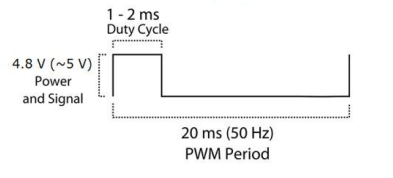
\includegraphics[scale=0.60]{figures/dutycycle.png}
				\caption{Servo Duty Cycle}
			\end{figure}
			\begin{itemize}
				\item[]PWM Signal:\\
				The servo is controlled using a PWM signal, which consists of a series of pulses. The width of each pulse determines the position of the servo. In this case, the pulse width ranges from 1 ms to 2 ms, corresponding to different servo positions.	The specific pulse width of 1.5 ms typically represents the neutral or center position of the servo.
				\item[] PWM Period:\\
					The PWM period is the time interval between the start of two consecutive pulses. In the datasheet, the PWM period is labeled as 20 ms (50 Hz).	This means that the servo receives a new position signal every 20 ms.
				\item[] Deadline (D):\\
					The deadline is the maximum allowed time for the servo to reach its desired position after receiving the PWM signal. In the context of servo control, the deadline is typically set to be slightly longer than the PWM period to allow for the servo's physical movement. From the image, we can infer that the deadline is set to 21 ms, which is 1 ms longer than the PWM period of 20 ms. This extra 1 ms provides a small buffer for the servo to complete its movement before the next PWM signal arrives.
				\item[] Period (T):\\
					The period represents the time interval at which the servo control task is executed. In this case, the period is chosen to be 100 ms, which is a multiple of the PWM period. A period of 100 ms means that the servo control task runs every 100 ms, allowing for multiple PWM signals to be sent within each control cycle. This period is selected based on the required responsiveness and smoothness of the servo movement.
				\item[] Execution Time (C):\\
					The execution time (C) is the time taken by the servo control task to generate and send the PWM signal to the servo. In the given scenario, the execution time is estimated or measured to be 20 ms. This execution time includes the time required for any calculations, signal generation, and communication overhead. It is important to ensure that the execution time is less than the deadline (D) to guarantee that the servo receives the control signal within the expected time frame.
			\end{itemize}





			\begin{figure}[H]
				\centering
				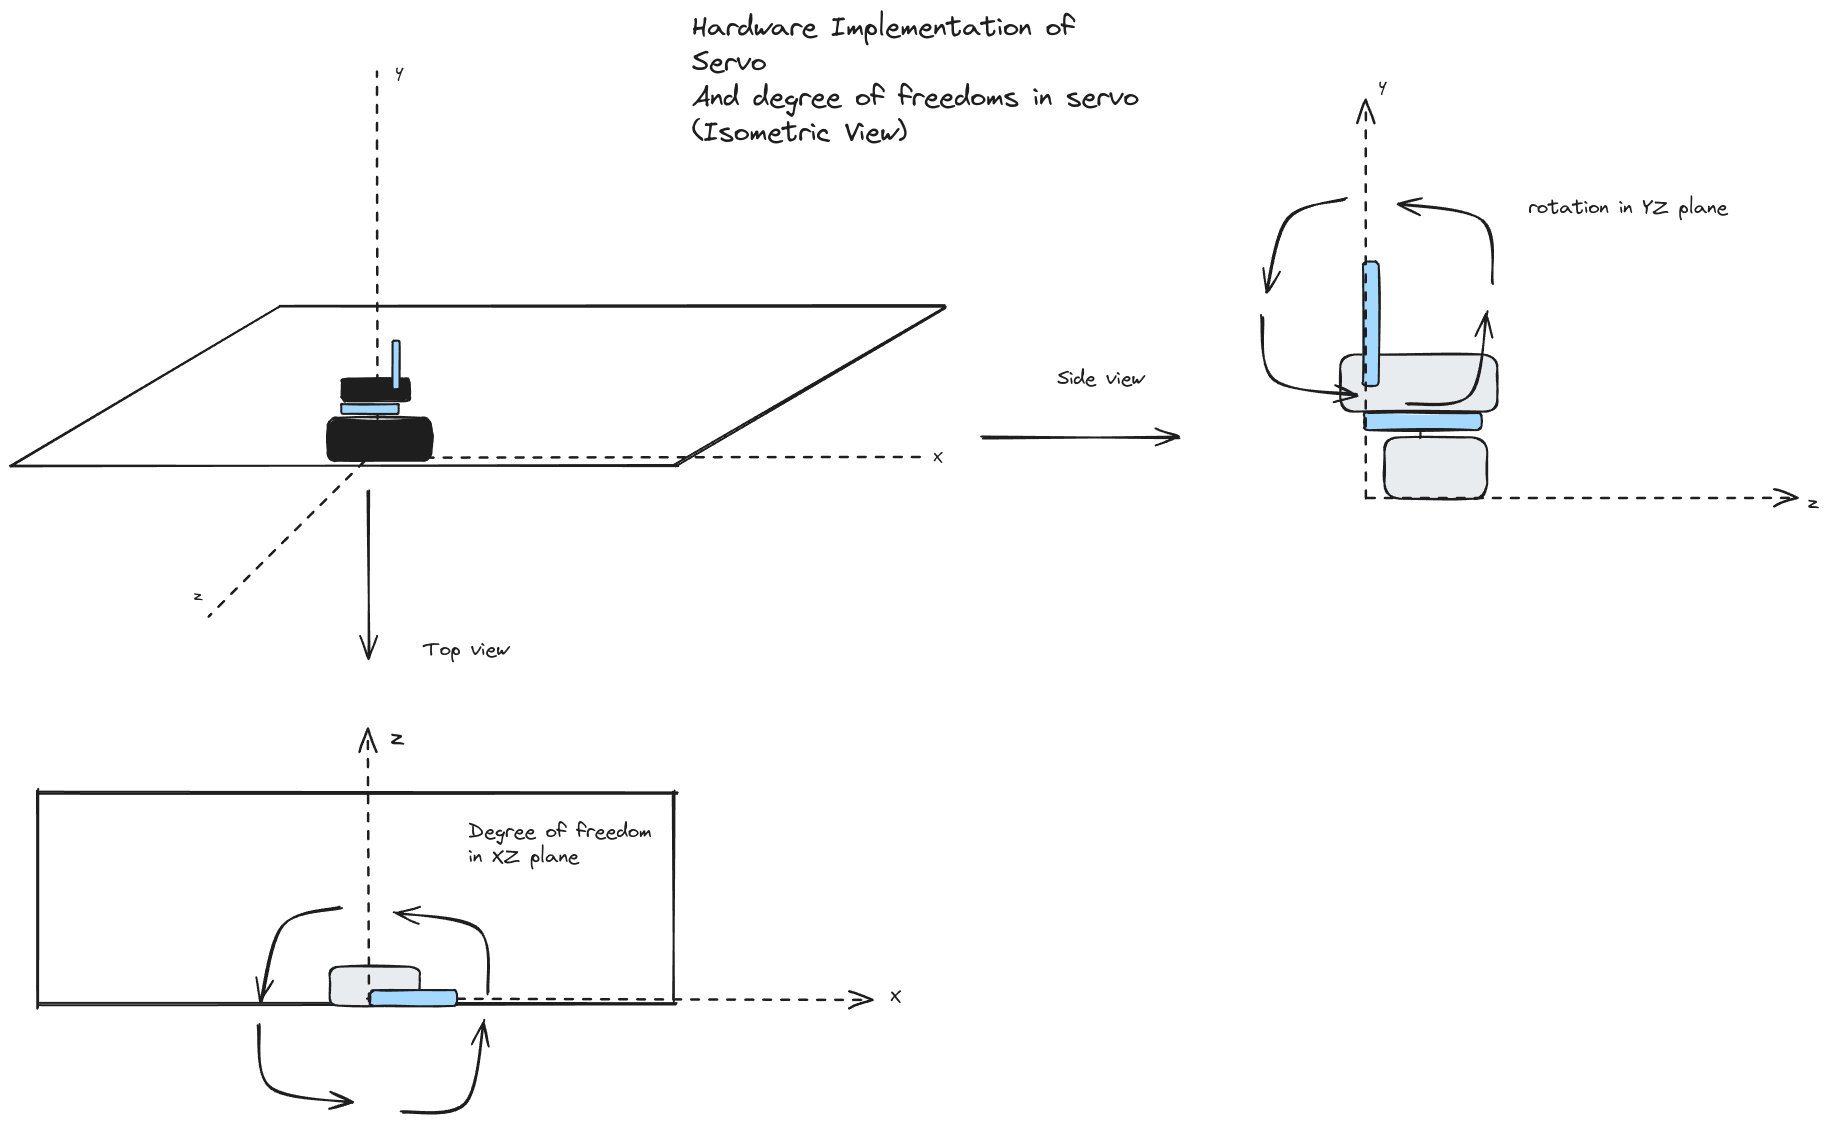
\includegraphics[scale=0.27]{figures/isometric.png}
				\caption{Different Views for Servo movement}
			\end{figure}


			\begin{itemize}
				\item[]Degree of Freedom in the XZ Plane:\\
				The servo at the base, represented in the bottom diagram as rotating in the horizontal plane, allows the system to pivot left and right. This rotation changes the orientation of the attached device along the X-axis (horizontal axis) and the Z-axis (depth axis). This movement is used for aiming the camera horizontally across a plane parallel to the ground.

				\item[]Rotation in the YZ Plane:\\
				The servo represented in the top-right diagram is mounted perpendicularly to the first servo and allows the system to tilt up and down. This tilting motion adjusts the orientation of the camera along the Y-axis (vertical axis) and the Z-axis. This type of movement is used to change the elevation angle of the device, pointing it up or down.
			\end{itemize}




			\begin{figure}[H]
				\centering
				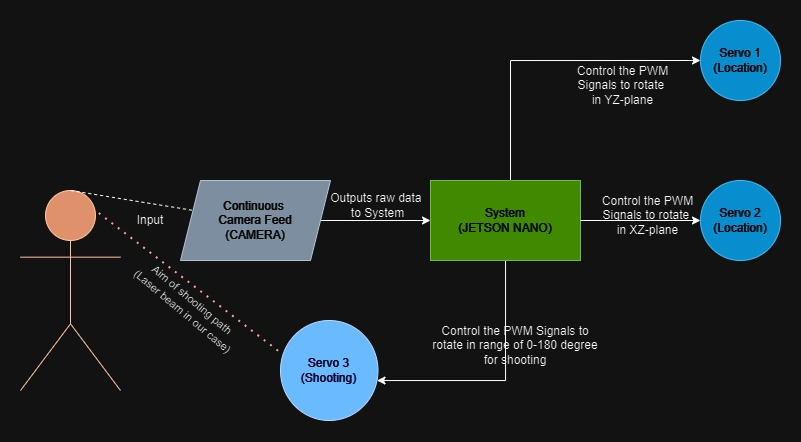
\includegraphics[scale=0.6]{figures/hw_overview.jpeg}
				\caption{Working Overview}
			\end{figure}
			\begin{itemize}
				\item Input - Continuous Camera Feed (CAMERA): The system begins with a camera that continuously captures video. This camera represents the primary sensor input for the system, continuously providing raw visual data.
				\item System (JETSON NANO): The raw camera feed is sent to the central processing unit, which is a Jetson Nano in this case. It processes the input data to detect faces and then calculates the necessary movements for the servo motors to align with the detected face.
				\item Servo 1 (Location): Based on the processed data from the Jetson Nano, Servo 1 adjusts the system's orientation in the YZ-plane (vertical plane). Control of the PWM (Pulse Width Modulation) signals to rotate in the YZ-plane suggests that Servo 1 can tilt the mechanism up or down to align vertically with the detected face.
				\item Servo 2 (Location): Simultaneously, Servo 2 receives control signals from the Jetson Nano to rotate in the XZ-plane (horizontal plane). This servo is responsible for the left-right movement, aligning the system horizontally with the target.
				\item Servo 3 (Shooting): Once the target is located and centered using Servos 1 and 2, Servo 3 is actuated. This servo controls the firing mechanism, and the diagram specifies that it can rotate in a range of 0-180 degrees to shoot, which implies a range of motion for the actuation mechanism, potentially to vary the firing angle or to engage a safety lock mechanism.
				\item The arrows indicate the direction of data and control flow. Starting from the camera input, moving to processing and decision-making on the Jetson Nano, and finally to the actuation of Servo 1 and Servo 2 for location alignment, and Servo 3 for shooting upon successful alignment.
			\end{itemize}


			\begin{figure}[H]
				\centering
				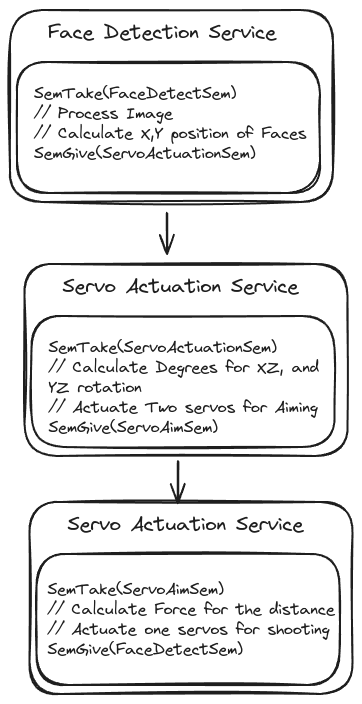
\includegraphics[scale=0.40]{figures/dataflow.png}
				\caption{Dataflow Diagram :DFD}
			\end{figure}
			\begin{itemize}
				\item[]Face Detection Service: This service is responsible for detecting faces in images captured by the system.It receives input from a function called SemTake(FaceDetectSem), which suggests the presence of a synchronization mechanism (semaphore) to control access to the face detection service.The service processes the image, performs face detection, and calculates the X,Y position of the detected faces.
				After processing, it releases the semaphore using SemGive(ServoActuationSem), indicating that the face detection results are ready for the next service.
				\item[] Servo Actuation Service:
					This service receives the face detection results from the Face Detection Service through the SemTake(ServoActuationSem) function. It calculates the necessary degrees for the X and Y axes to aim the servos towards the detected face. Based on the calculated degrees, it actuates two servos using the SemGive(ServoAimSem) function, which suggests passing control to the Servo Aiming Service.
				\item[] Servo Aiming Service:
					This service takes control after receiving the signal from the Servo Actuation Service through SemTake(ServoAimSem).It calculates the force required to aim the servos based on the distance to the detected face.Finally, it actuates one servo for shooting, likely triggering a shooting mechanism.After the shooting action, it releases the control back to the Face Detection Service using SemGive(FaceDetectSem).
			\end{itemize}
			The arrows in the diagram represent the flow of control and data between the services. The use of semaphores (SemTake and SemGive) suggests a synchronization mechanism to ensure that each service operates in a coordinated manner and that data is passed correctly between them.


	\end{enumerate}
	\section{Question 6}
	\begin{enumerate}
		\item[] \Q [10 points] Provide all major real-time service requirements with a description of each
			Si including Ci, Ti, and Di with a description of how the request frequency and deadline was
			determined for each as well as how Ci was determined, estimated or measured as WCET for
			the service. Deadlines must be real and related to a published standard; or physical
			requirement based on mathematical modeling; or research paper or study. Please provide this
			in your report for the final project as well as your Exercise 6 submission.
			\A \textbf{Service 1 (S1): Face Detection}\\
			Description: The face detection service captures video frames from the camera, detects faces in each frame using computer vision algorithms, and extracts the coordinates of the detected faces.
			\begin{figure}[H]
				\centering
				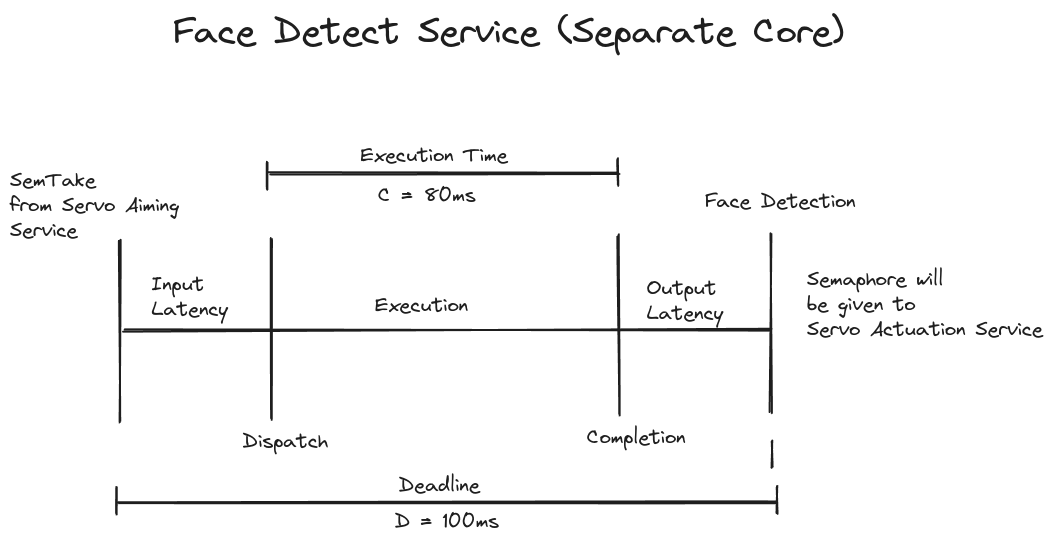
\includegraphics[scale=0.4]{figures/face_detect_service.png}
				\caption{Face Detect Service Analysis}
			\end{figure}
			\textbf{This service would run on different core than Servo Actuation and Servo Aiming Service}
			\begin{itemize}
				\item[]Execution Time (C1): 80 milliseconds\\
				The period was chosen based on the requirement to process video frames at a rate of 10 frames per second (FPS) to achieve smooth and responsive face tracking. A period of 100 milliseconds ensures that the face detection service can process each frame within the allocated time.
				\item[] Deadline (D1): 100 milliseconds\\
					The deadline for the face detection service is set to be equal to its period (D1 = T1) to ensure that the processing of each frame is completed before the next frame arrives. This deadline is derived from the real-time requirement of processing video frames at 10 FPS for seamless face tracking.
				\item[] Period (T1): 100 milliseconds\\
					The period was chosen based on the requirement to process video frames at a rate of 10 frames per second (FPS) to achieve smooth and responsive face tracking. A period of 100 milliseconds ensures that the face detection service can process each frame within the allocated time.
			\end{itemize}


			\textbf{Service 2 (S2): Servo Control}\\
			\begin{figure}[H]
				\centering
				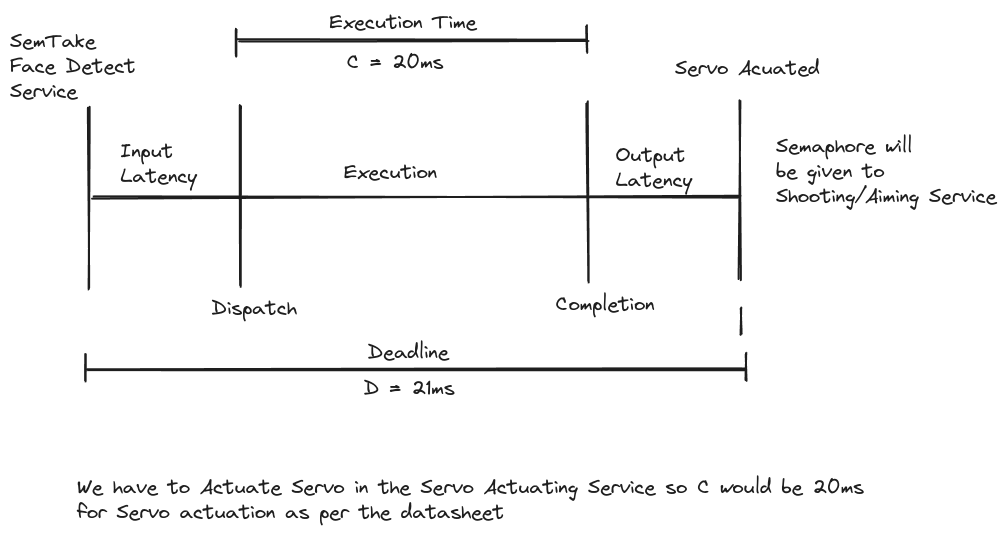
\includegraphics[scale=0.4]{figures/servo_actuation_service.png}
				\caption{Servo Actuation Service Analysis}
			\end{figure}
			Description: The servo control service receives the face coordinates from the face detection service, calculates the required servo angles using trigonometric calculations, and sends control signals to the servos to aim at the detected face.
			\begin{itemize}
				\item[] Execution Time (C2): 20 milliseconds
					The execution time for the servo control service was determined by measuring the WCET of the servo angle calculation and control signal generation on the Jetson Nano platform. The WCET was obtained by considering the maximum time required for the trigonometric calculations and servo communication.
				\item[] Period (T2): 100 milliseconds
					The period for the servo control service is set to 21 milliseconds to ensure smooth and responsive servo movement. This period allows the servos to update their positions frequently enough to track the detected face accurately.
				\item[] Deadline (D2): 21 milliseconds
					The deadline for the servo control service is to guarantee that the servo angles are calculated and control signals are sent within the allocated time. This deadline ensures that the servos can respond quickly to changes in the face position.
			\end{itemize}


			\textbf{Service 3 (S3): Shooting Mechanism Control}\\
			\begin{figure}[H]
				\centering
				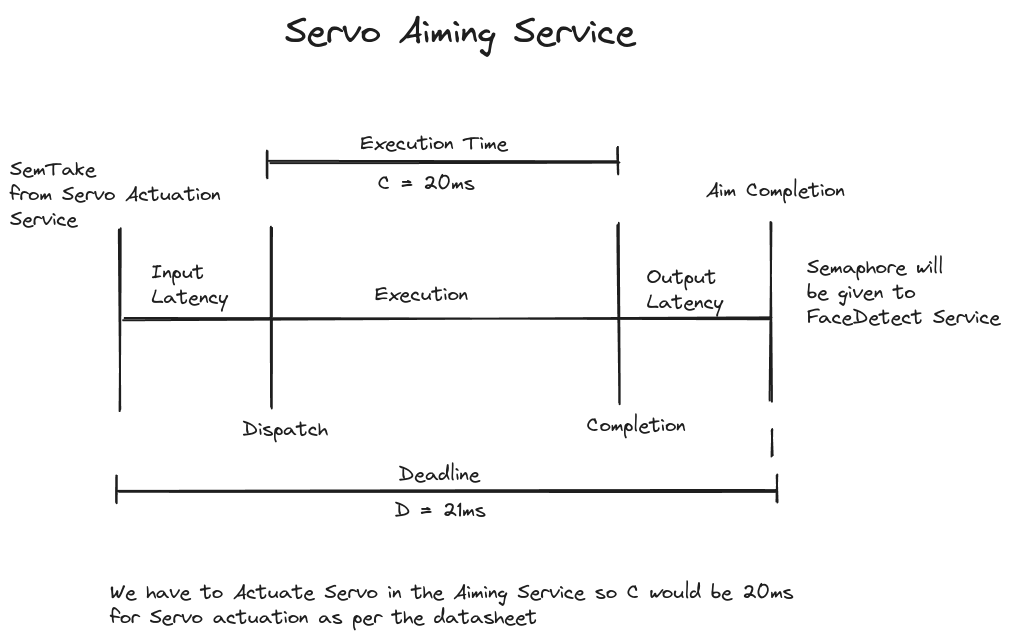
\includegraphics[scale=0.4]{figures/servo_aiming_service.png}
				\caption{Servo Aiming Service Analysis}
			\end{figure}
			Description: The shooting mechanism control service monitors the alignment between the servos and the detected face, and triggers the shooting action when the alignment conditions are met.
			\begin{itemize}
				\item[] Execution Time (C3): 20 milliseconds
					The execution time for the shooting mechanism control service was determined by measuring the WCET of the alignment check and trigger signal generation on the Jetson Nano platform. The WCET was obtained by considering the maximum time required for the alignment calculations and shooting mechanism communication.
				\item[] Period (T3): 100 milliseconds
					The period for the shooting mechanism control service is set to 100 milliseconds, aligning with the face detection service's period. This period allows the shooting mechanism to be triggered in sync with the face detection and tracking process.
				\item[] Deadline (D3): 21 milliseconds
					The deadline for the shooting mechanism control service is set to be equal to its period (D3 = T3) to ensure that the alignment check and trigger signal generation are completed within the allocated time. This deadline guarantees that the shooting mechanism can respond promptly to the detected face alignment.
			\end{itemize}

			\begin{table}[H]
				\centering
				\begin{tabular}{l l c c c c}
					\hline
					\textbf{Service} & \textbf{Service name}    & \textbf{C} & \textbf{WCET} & \textbf{D} & \textbf{T} \\\hline
					                 &                          &                                                      \\
					S1               & Face Recognition Service & 80ms       & 100ms(??)     & 100ms      & 100ms      \\
					S2               & Servo Actuation Service  & 20ms       & 20ms(??)      & 21ms       & 100ms      \\
					S3               & Servo Aiming Service     & 20ms       & 20ms(??)      & 21ms       & 100ms      \\

					\hline\hline
				\end{tabular}
				\caption{Estimated C,D,T}
			\end{table}

	\end{enumerate}

	\pagebreak

	\section{References}
	\begin{enumerate}
		\item ECEN 5623 Lecture slides material and example codes.
		\item REAL-TIME EMBEDDED COMPONENTS AND SYSTEMS with LINUX and RTOS, Sam Siewert John
		      Pratt (Chapter 10, 11 \& 12).
		\item Exercise 6 requirements included links and documentation.
	\end{enumerate}

	\bibliographystyle{plainnat}
	\bibliography{references}


\end{qanda}




\vfill
\hrule
\vspace{0.5cm}
\pagebreak
\begin{appendices}
	\section{C Code for the Implementation}
	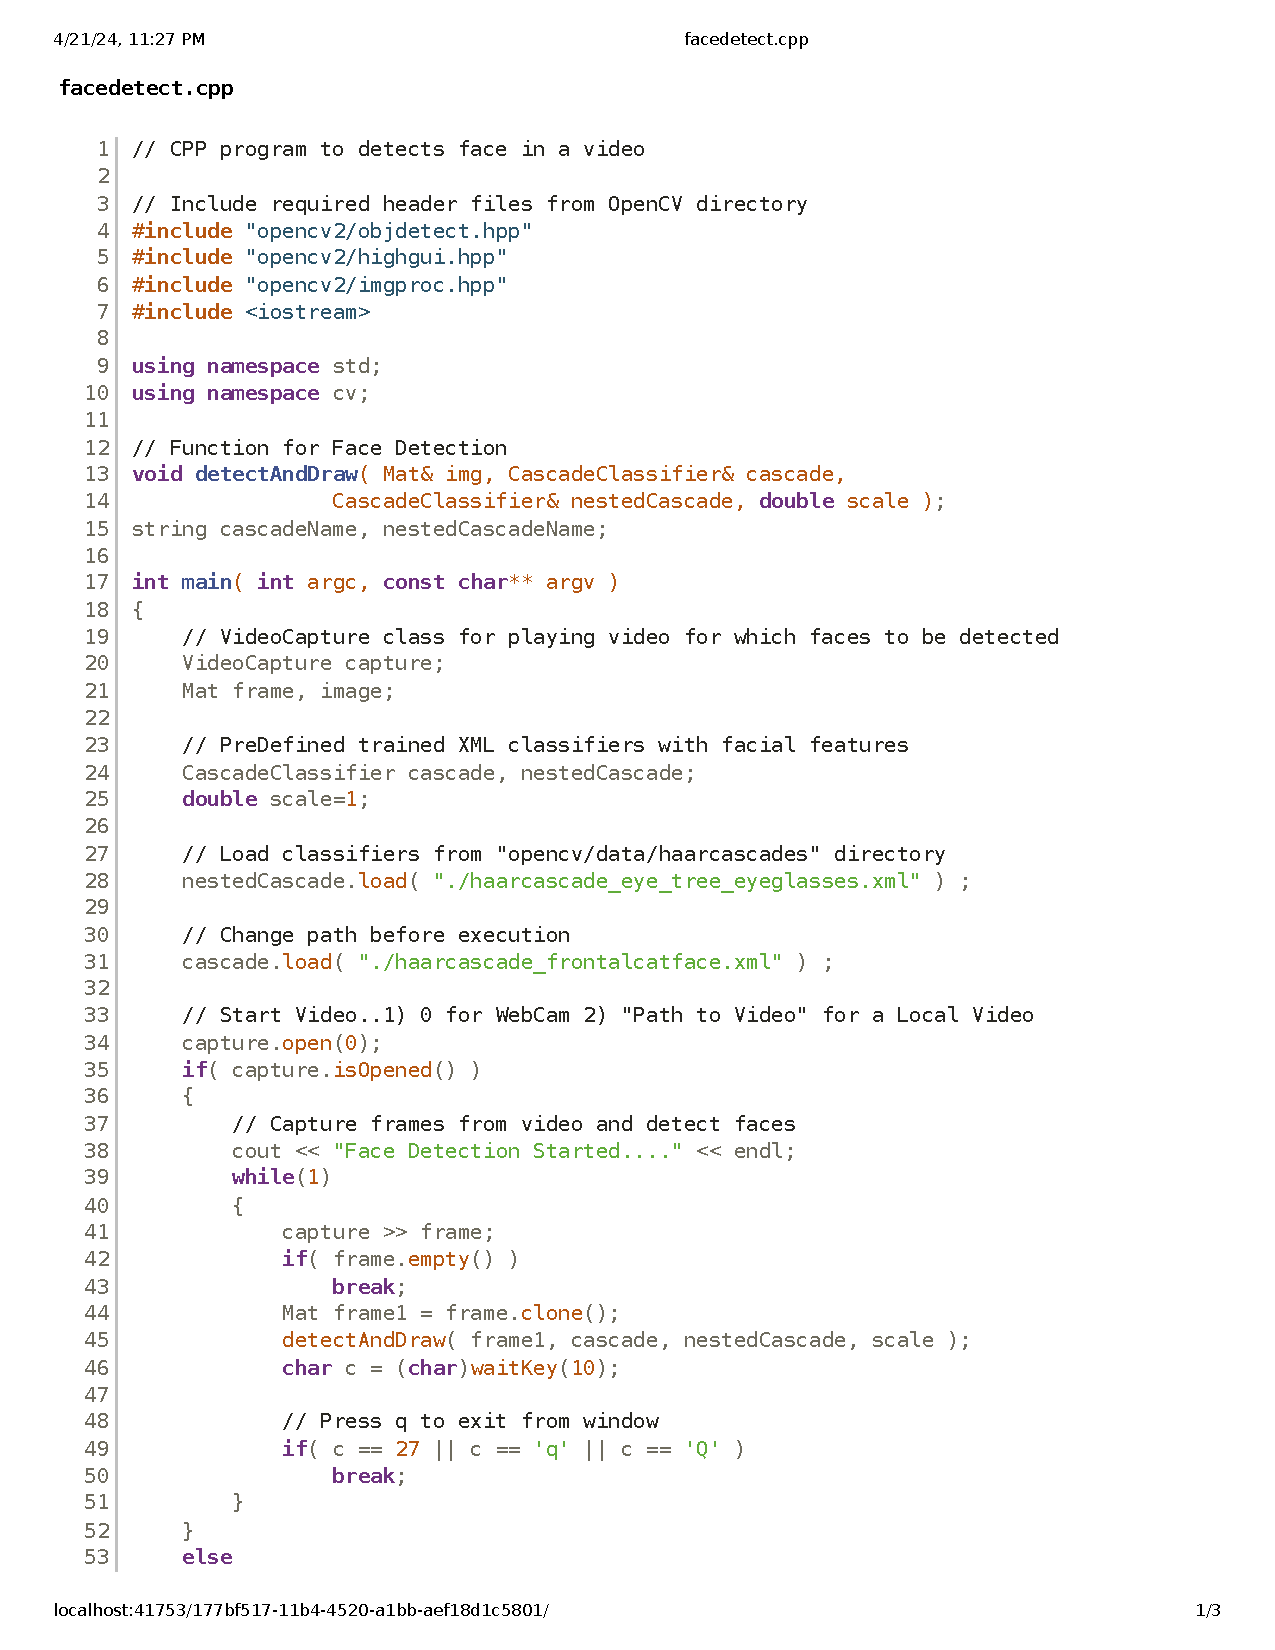
\includepdf[pages=-]{code/facedetect.cpp.pdf}
	\pagebreak
\end{appendices}


\vspace{1cm}
\hrule
\vspace{0.5cm}


%---------------------------------------------------------------------------
\end{document}
-
